\documentclass[12pt]{article}

\usepackage{fullpage}
\usepackage{multicol,multirow}
\usepackage{tabularx}
\usepackage{listings}
\usepackage[utf8]{inputenc}
\usepackage[russian]{babel}
\usepackage{graphicx}
\usepackage{csquotes}

\begin{document}

\begin{titlepage}

    \begin{center}

        \bfseries
        {\small Московский авиационный институт\\ 
        (национальный исследовательский университет)}

        % \vspace{48pt}
        {\small Факультет информационных технологий и прикладной 
        математики}
        
        % \vspace{36pt}
        {\small Кафедра вычислительной математики и программирования}
        
        \vspace{8cm}
        {\Large Лабораторная работа \textnumero 3 по курсу} 
        \enquote{\Large Компьютерная графика}
        
    \end{center}
    
    \vspace{84pt}
    \begin{flushright}
        \begin{tabular}{rl}
            Студент: & Е.Ю. Юрков \\
            % Преподаватель: &  \\
            Группа: & М80-312Б-22 \\
            Дата: & \\
            Оценка: & \\
            Подпись: & \\
        \end{tabular}
    \end{flushright}
    
    \vfill
    
    \begin{center}
        
        \bfseries
        Москва, \the\year
    
    \end{center}

\end{titlepage}

% Выполнил студент группы М8О-312Б-22 МАИ \textit{Юрков Евгений}.

\subsection*{Цель лабораторной работы}

В этой лабораторной работе вы научитесь работать с камерой в 3D-пространстве,
управлять её положением и направлением, а также освоите базовые трансформации
(перемещение, поворот и масштабирование) объектов в 3D.

\subsection*{Задача}

\textbf{Вариант 7. Комбинация трансформаций (перемещение, масштабирование, поворот)}

Постройте несколько объектов (например, куб и пирамиду) в разных местах сцены.
Реализуйте для каждого объекта возможность перемещения, масштабирования и
поворота.
Управление должно осуществляться через клавиатуру, при этом трансформации должны
применяться последовательно.

% \newpage
\subsection*{Метод решения}

Для выполнения лабораторной работы я изменил код предыдущей работы добавив к классам объектов
(кубу, сфере, пирамиде) метод transform, который получает матрицу модели и преобразует фигуру с помощью неё.

Перемещение объектов происходит с помощью клавиш W,A,S,D, поворот с помощью клавиш I,J,K,L, а масштабирование
с помощью Ctrl и Space.

\subsection*{Результат работы программы}

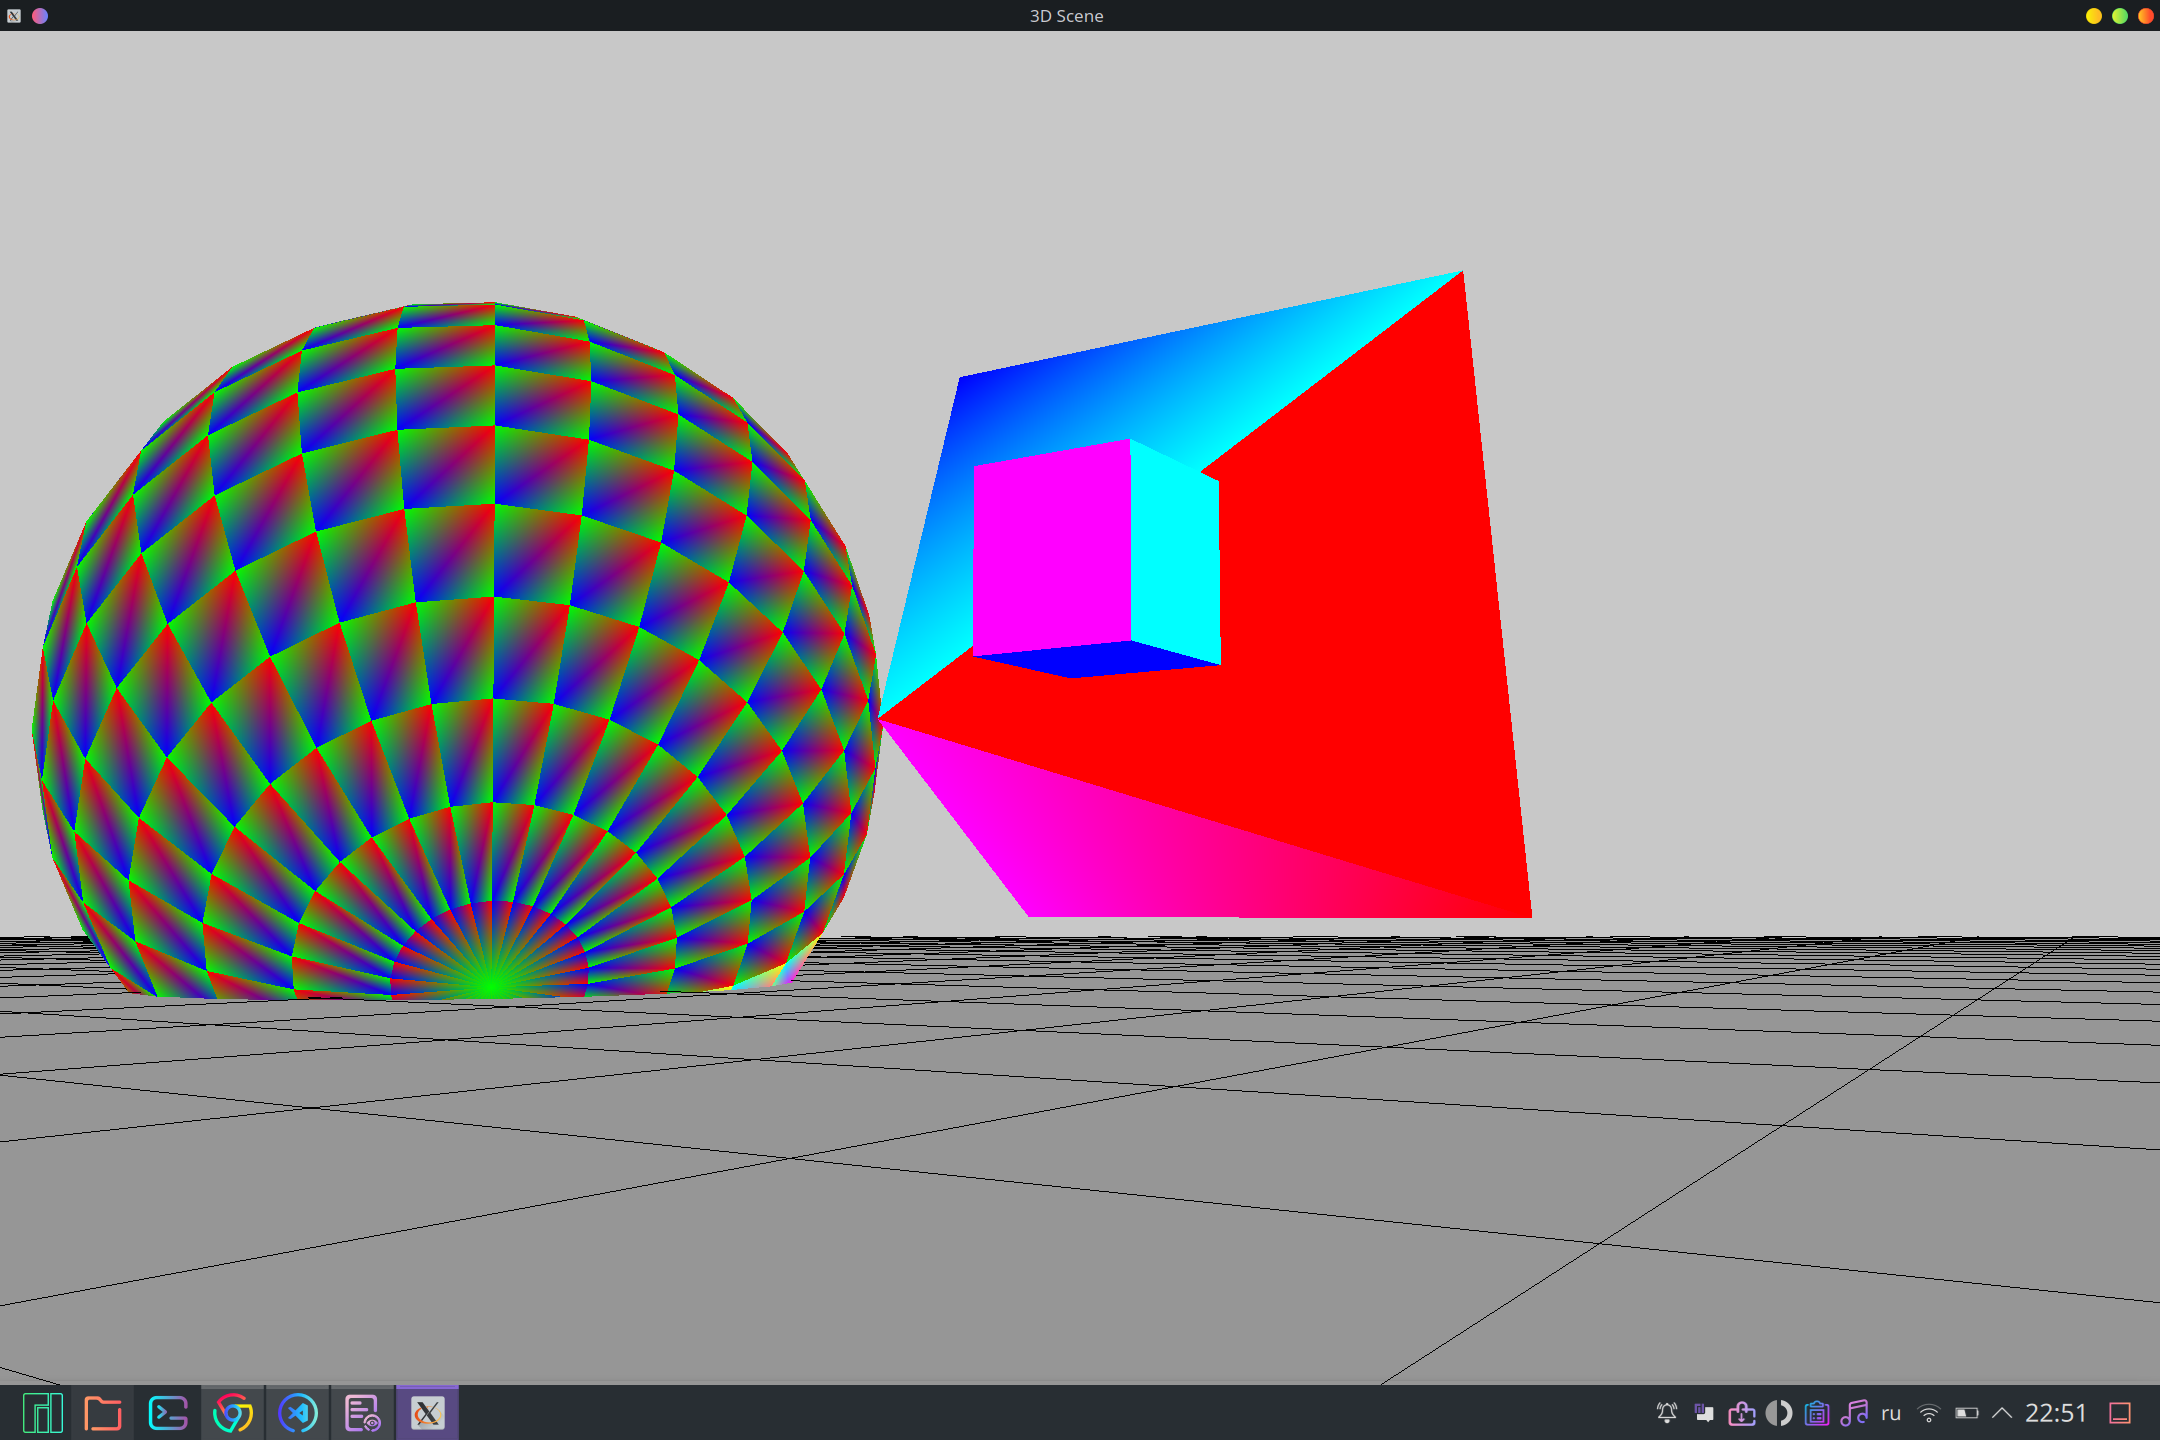
\includegraphics[width=15cm]{demo.png}

% \newpage
\subsection*{Выводы}

В процессе выполнения лабораторной работы я применил знания о преобразованиях объектов,
полученные в первой лабораторной работе для трёхмерных объектов, а также углубил знания
о настройке взаимодействия с пользователем через клавиатуру и мышь.

\end{document}